\section{Theory}\label{sec:theory}
\subsection{Gaussian Distribution}
The gaussian distribution or the normal distribution is an important distribution that is often used in natural and social sciences for real-valued random variables when their distributions are not known. The importance of this distribution comes from the central limit theorem, that states for any under some conditions the average of many (enough) observations of a random variable with finite mean and variance converges to a normal distribution even if the random variable comes from another distribution.\cite{WikipediaGaussian}. The most important thing here is that the probability density function of a normal distribution with mean $\mu$ and variance $\sigma^2$ is
\begin{equation}
	f(x) = \frac{1}{\sqrt{2\pi\sigma^2}}e^{-\frac{1}{2}(\frac{x-\mu}{\sigma})^2}
\end{equation}
which gives the probability to obtain any value $x\in\mathbb{R}$ from this distribution.\\
In this particular project we use the complex gaussian distribution which for our random variables has the probability density function
\begin{equation}
	f(x) = \frac{1}{\pi\sigma^2}e^{-\frac{1}{\sigma^2}|x-\mu|^2}
\end{equation}
Which in this case take in any value $x\in\mathbb{C}$
\subsection{Estimators}
When we with probable cause can say something about the distribution that the random variables are sampled from, but not their mean and/or variance, we can estimate these distributions properties. Assumed that the random variables are sampled independent from the same identical distribution (iid), then the mean can be estimated with the average of the samples, which is unbiased.
\begin{align}
	\hat{\mu} & = \mathbb{E}\{\frac{1}{N}\sum_{n=0}^{N-1}x\}\nonumber\\
	& = \frac{1}{N}\sum_{n=0}^{N-1}\mathbb{E}\{x\}\nonumber\\
	& = \frac{1}{N}\sum_{n=0}^{N-1}\mu\nonumber\\
	& = \mu\label{eq:mu_est}
\end{align}
Meaning that the expected value of the mean of the samples will, with the number of samples taken, converge to the actual expected value of the distribution.\\
This is also the case if there are samples of the variance of the data available
\begin{align}
	\hat{\sigma^2} & = \mathbb{E}\{\frac{1}{N}\sum_{n=0}^{N-1}\sigma^2\}\nonumber\\
	& = \frac{1}{N}N\sigma^2\nonumber\\
	& = \sigma^2\label{eq:sigma_est}
\end{align}
These two results are used when solving the problems later on in this report.
\subsection{(Binary) Hypothesis Testing}
Detection problems are often formulated to be about if a signal is present or not in conditions which masks the signal that we desire to detect, for instance white gaussian noise. The hypothesises that could be formulated is:
\begin{align}
\begin{split}
	\text{Null hypothesis} H_0 &: x[n] \thicksim \mathbb{P}_0\\
	\text{Alternative hypothesis} H_1 &: x[n] \thicksim \mathbb{P}_1
\end{split}
\end{align}\label{eq:gen_hypothesis_test}
where the null hypothesis is ''no signal present'' and alternative hypothesis is ''signal present'', and $\mathbb{P}_0$ and $\mathbb{P}_1$ are two arbitrary distributions.\\
Let $[x[0] x[1] \dots x[N-1]]$ be sampled random variables from a sensor where it is constant "1" when detecting an object and constant "0" when not detecting anything. A simple detector in this case could be by setting a threshold at $\lambda = 0.3$ that detects when the threshold is broken. The problem with this simple detector appears when the signal from our sensor is noisy.\\
Let now the samples from our sensor be
\begin{align}
	H_0 &: x[n] = w[n]\nonumber\\
	H_1 &: x[n] = A + w[n]\nonumber
\end{align}
where $w[n] ~ \mathcal{N}(0, 1)$. Then under the null hypothesis in a non-noisy environment $w[n] = 0 \implies x[n] = 0$, however we have a noisy envirnoment so $x[n]$ obtains random values from the normal distribution with zero mean and unit variance. In figure \ref{fig:noise} we can see how the data we obtain from 100 samples may look like.
\begin{figure}
	\centering
	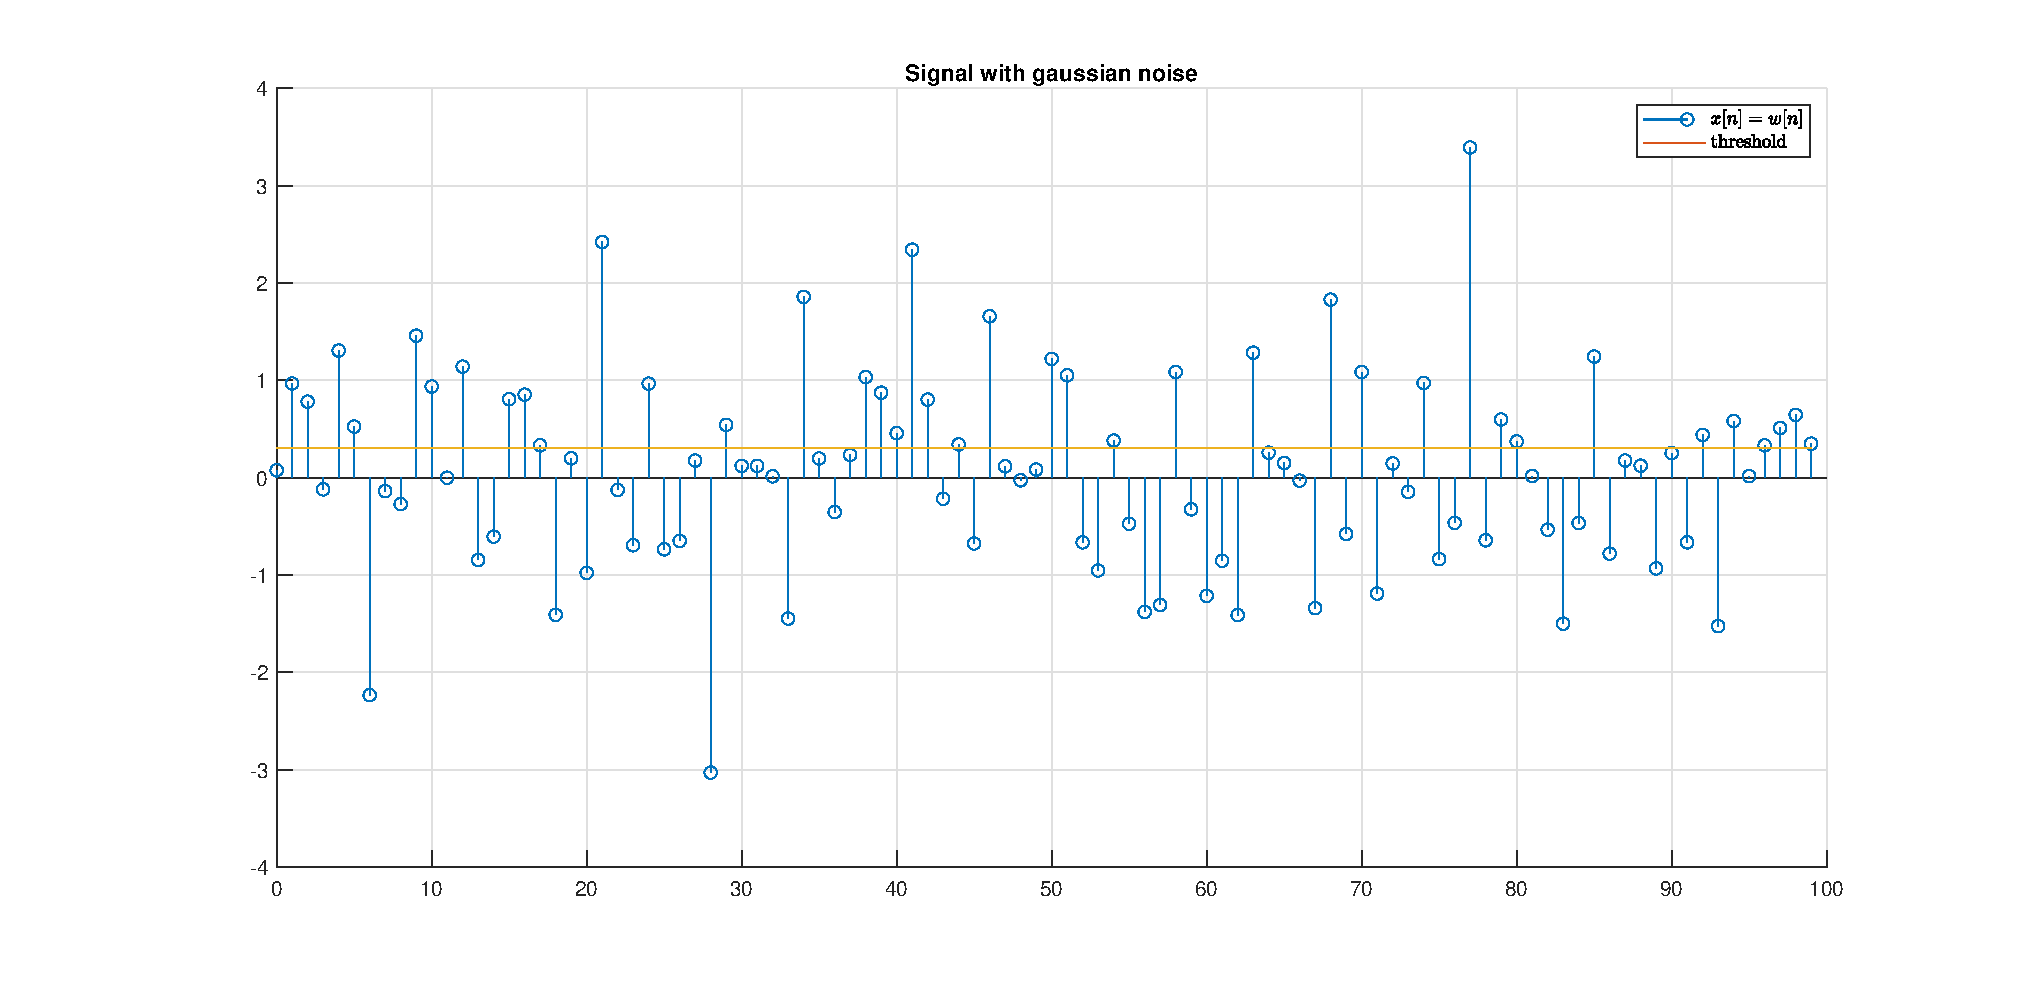
\includegraphics[width = \linewidth]{figures/gen_sign_noise.eps}
	\caption{100 samples from a gaussian distribution $\mathcal{N}(0,1)$}
	\label{fig:noise}
\end{figure}
From these 100 samples there are 39 samples that are above the set threshold meaning that from these 100 samples we will get 39 false positives/alarms which will alert the user that there is an object detected when there really is not. Our goal when solving detection problems is to develop a detector that from the samples can find a decision rule so that the number of false alarms is minimized but at the same time manages to detect correctly when there is an object present.\cite{Myrvoll2020}\\
\subsection{Neyman-Pearson detector}
The Neyman-Pearson detector utilizes the likelihood ratio test (LRT)
\begin{equation}
	L(\mathbf{x}) \triangleq \frac{p_1(\mathbf{x})}{p_0(\mathbf{x})} 
		\begin{cases}
			\geq \lambda \implies H_1
			< \lambda \implies H_0
		\end{cases} 
\end{equation}
where $p_1(x)$ and $p_0(x)$ is the point distribution functions or the likelihood functions of the distributions under $H_1$ and $H_0$ respectively.
With the Neyman-Pearson detector the threshold $\lambda$ is chosen to satisfy the constraint and to maximize the power such that
\begin{equation}
	P_{FA} = \alpha = \int_{L(\mathbf{x})>\lambda}p_0(\mathbf{x})d\mathbf{x}
\end{equation}
where $\alpha_0$ the tuning factor. This goes hand in hand with the detection rate of the detector as well since the Neyman-pearson lemma states that to increase the power of the likelihood ratio test, the false alarm rate is also increased. \todo{Mye dårlige formuleringer her. Må skrives om}
\begin{enumerate}[i]
	\item \underline{Inform} the reader that this chapter is a presentation of the theory needed to understand the task
	\item You may copy parts from lecture notes (but inform
	the reader that you have done this!). Also refer to
	books in former courses or other literature
	\begin{itemize}
		\item Always refer to the source and
		\item Use quotation marks when quoting (copying) 
	\end{itemize}
	\item Use figures if possible/natural!
\end{enumerate}